%                                                                 aa.dem
% AA vers. 8.2, LaTeX class for Astronomy & Astrophysics
% demonstration file
%                                                       (c) EDP Sciences
%-----------------------------------------------------------------------
%
%\documentclass[referee]{aa} % for a referee version
%\documentclass[onecolumn]{aa} % for a paper on 1 column  
%\documentclass[longauth]{aa} % for the long lists of affiliations 
%\documentclass[rnote]{aa} % for the research notes
%\documentclass[letter]{aa} % for the letters 
%\documentclass[bibyear]{aa} % if the references are not structured 
% according to the author-year natbib style

%
\documentclass[letter]{aa}  

%
\usepackage{graphicx}
%%%%%%%%%%%%%%%%%%%%%%%%%%%%%%%%%%%%%%%%
\usepackage{txfonts}
%%%%%%%%%%%%%%%%%%%%%%%%%%%%%%%%%%%%%%%%
\usepackage{tabularx}
\usepackage{amsfonts}
\usepackage{bbold}
\usepackage{color}
\usepackage{transparent}
\usepackage{hyperref}
\usepackage{transparent}
\usepackage{rotating}
\usepackage{caption}
\usepackage{subcaption}

% Only include extra packages if you really need them. Common packages are:
\usepackage{graphicx}	% Including figure files
\usepackage{amsmath}	% Advanced maths commands
\usepackage{amssymb}	% Extra maths symbols
\usepackage{tablefootnote}
\usepackage[flushleft]{threeparttable}
\usepackage{dblfloatfix} 

\usepackage{natbib}
\bibpunct{(}{)}{;}{a}{}{,} 

\newcommand{\sgx}{SgXB\xspace}
\newcommand{\ulx}{ULX\xspace}
\newcommand{\sfxt}{SFXT}
\newcommand{\sg}{Sg\xspace}
\newcommand{\co}{CO\xspace}
\newcommand*{\hmxb}{HMXB\@\xspace}
\newcommand*{\lmxb}{LMXB\@\xspace}
\newcommand*{\rlof}{RLOF\@\xspace}
\newcommand*{\ns}{NS\@\xspace}
\newcommand*{\bh}{BH\@\xspace}
\newcommand*{\eg}{e.g.\@\xspace}
\newcommand*{\ie}{i.e.\@\xspace}
\newcommand*{\aka}{a.k.a. \@\xspace}
\newcommand*\diff{\mathop{}\!\mathrm{d}}
\newcommand{\mystar}{{\fontfamily{lmr}\selectfont$\star$}}
\newcommand*{\msun}{$M_{\odot}$\@\xspace}
\newcommand*{\mdotstar}{$\dot{M}_{\text{\mystar}}$\@\xspace}
\newcommand*{\mdotacc}{$\dot{M}_{\text{acc}}$\@\xspace}
\newcommand*{\ledd}{$L_{\text{Edd}}$\@\xspace}

 
%\usepackage[options]{hyperref}
% To add links in your PDF file, use the package "hyperref"
% with options according to your LaTeX or PDFLaTeX drivers.
%
\begin{document} 


   \title{Mass transfer via wind-RLOF in Supergiant X-ray binaries}

   \subtitle{A possible mechanism for Ultraluminous X-ray sources}

   \author{I. El Mellah
          \inst{1}
          \and
          J. O. Sundqvist
          \inst{2}
          \and
          R. Keppens
          \inst{1}
          }

   \institute{Centre for mathematical Plasma Astrophysics, 
   			 Department of Mathematics, KU Leuven, 
   			 Celestijnenlaan 200B, B-3001 Leuven, Belgium\\
              \email{ileyk.elmellah@kuleuven.be}
         \and
             KU Leuven, Instituut voor Sterrenkunde, 
             Celestijnenlaan 200D, B-3001 Leuven, Belgium
             }

   \date{Received ...; accepted ...}

% \abstract{}{}{}{}{} 
% 5 {} token are mandatory
 
  \abstract{Ultra-luminous X-ray sources (\ulx) have such high X-ray luminosities that they were long thought to be accreting intermediate mass black holes. Yet, some have been shown to display periodic modulations and coherent pulsations, suggestive of a neutron star in orbit around a companion and accreting at super-Eddington rates. The question of the mass transfer mechanism suitable to feed the accretor at such high rates remains open. In this letter, we propose that Supergiant X-ray binaries (\sgx) could undergo a \ulx phase when the slow line-driven wind from the hot donor star is highly beamed towards the compact accretor. Since the star does not fill its Roche lobe and that a significant fraction of the stellar wind still escapes the system, this mass transfer mechanism known as "wind - Roche lobe overflow" can remain stable even for large mass ratios. Based on line-acceleration profiles derived from spectral observations and modeling of the stellar wind, we perform three-dimensional ballistic simulations to evaluate the fraction of the wind captured by the compact object. We identify realistic orbital and stellar conditions for a \sgx to be the stage of mass transfer rates matching the expectations for \ulx and show that the transition from \sgx to \ulx luminosity levels is progressive. These results prove that high stellar Roche lobe filling factors are not necessary to funnel large quantities of material into the Roche lobe of the accretor. Slow and dense winds such as the ones emitted by the Wolf-Rayet star in M101 ULX-1 or even the cold Red Supergiant in P13 ULX-1 are enough to lead to a highly beamed wind and a significantly enhanced mass transfer rate.}

   \keywords{XXX accretion, accretion discs -- X-rays: binaries -- stars: neutron, supergiants, winds, outflows -- methods: numerical}

   \maketitle
%
%________________________________________________________________

XXX

notwithstanding
hitherto

XXX

\section{Introduction}

Ultra-luminous X-ray sources are point sources with luminosities in excess of 10$^{39}$erg$\cdot$s$^{-1}$ \citep[see][for a recent review]{Kaaret2017}. This X-ray luminosity threshold corresponds approximately to the Eddington luminosity \ledd of a 10\msun black hole (\bh), the limit above which isotropic accretion onto a body of this mass is thought to be self-regulated by the radiative field it produces \citep{Rappaport2005}. They are found off-nuclear in galaxies within a couple of 10Mpc, ruling against a supermassive black hole origin. If the emission is not beamed, such accretion rates can only be sustained for accretors of at least several 10 to several 100\msun bodies, suggestive of the long awaited population of intermediate mass black holes \citep{Colbert1999}. The observation of gravitational waves emitted by merging compact objects unearthed \bh of several 10\msun, while the accretors in the ULX IC 10 X-1 \citep{Brandt1997,Prestwich2007,Silverman2008} and M82 X-1 \citep{Brightman2016} are both 20 to 35\msun \bh. 

However, the detections of a cyclotron resonance scattering feature and of coherent pulsations from several ULX demonstrate that other ULX host super-Eddington accreting neutron stars \citep[\ns][]{Bachetti2014,Furst2016,Israel2017,Carpano2018,Brightman2018}. In one of them, NGC7793 P13 (hereafter P13), \cite{Motch2014} identified a stellar spectrum consistent with a 20\msun B9Ia star, in a $\sim$64 days orbit with an X-ray source they assumed to be a \bh but which later turned out to be an accreting \ns \citep{Furst2016}. It was further argued that the star has to fill its Roche lobe because the stellar mass loss rate would be too low and wind accretion would not be able to lead to a significant fraction of the stellar wind being captured by the accretor. Furthermore, \cite{Fuerst2018} isolated the intrinsic pulse period derivative which shows a strong spinning up of the accreting \ns. On the other hand, \citep{Liu2013} showed that in M101 ULX-1, the Helium emission lines are best explained by a Wolf-Rayet donor star twice smaller than its Roche lobe, ruling out the possibility of a mass transfer towards the accreting stellar mass \bh via Roche lobe overflow (\rlof). This result illustrates the pressing need for a better understanding of wind capture in binary systems.

The final absolute X-ray luminosity $L_X$ released by accretion onto a compact object fed by a stellar companion depends on :
\begin{itemize}
\item \mdotstar, the stellar mass loss rate which sets the maximum rate reachable.
\item $\dot{M}$, the rate at which mass is transferred from the star into the domain of gravitational influence of the accretor (either the Roche lobe or the accretion cylinder).
\item \mdotacc, the mass which actually ends up being accreted onto the compact object.
\item $\zeta$, the efficiency of the conversion of accreted mass to radiation. In this paper, we set it to 10$\%$, appropriate for negligible outflows \citep{Kaaret2017}.
\end{itemize} 
with \mdotstar$>\dot{M}>$\mdotacc. In this letter, we set aside the question of the mechanism responsible for super-Eddington accretion itself \ie how the compact object can accrete at a rate \mdotacc leading to $L_X>$\ledd. Rather, we  

 mechanism leading to super-Eddington accretion which explains how the compact object can accrete at a rate \mdotacc Pinto

Although another scenario is investigated in this letter.

Regardless of the mechanism which explains the super-Eddington accretion rates in the immediate vicinity of the accretor, which source of matter? Likely binary systems (natural extension of the HMXB LX distribution) where a donor star plays the role of a reservoir tapped by the orbiting compact object. In P13 for instance, high mass star + NS. In M101, the spectrum is suggestive of a WR star and the accretor might be a BH (Liu2013).

X-ray binaries have lower luminosities though. Neither RLOF nor wind BHL can reach these levels. RLOF, ~LMXB, limited by the transverse section of the channel @ L1 while fast winds (~HMXB) mean low capture cross-sections. The first is essentially limited by the small sound speed compared to the orbital speed while the second is limited by the large wind speed with respect to the orbital speed. => wind-RLOF configuration leading to enhanced accretion, best of both worlds when the stellar mass loss rate is large. \cite{King2002} suggested that above a mass ratio unity, unstable RLOF mass transfer occurs on a thermal time scale and lead to high mass accretion rate onto the compact companion. However, \cite{Pavlovskii2017} recently found that RLOF mass transfer can be stable for large q, up to 7.5. Not high enough though to match the mass ratio in P13 where the stellar mass is at least 10 times larger than the mass of the accreting \ns.

% ------------------------------------------------
\section{Line-driven wind acceleration in SgXB}
\label{sec:}
% ------------------------------------------------

\begin{figure}
\begin{subfigure}{.5\textwidth}
\centering
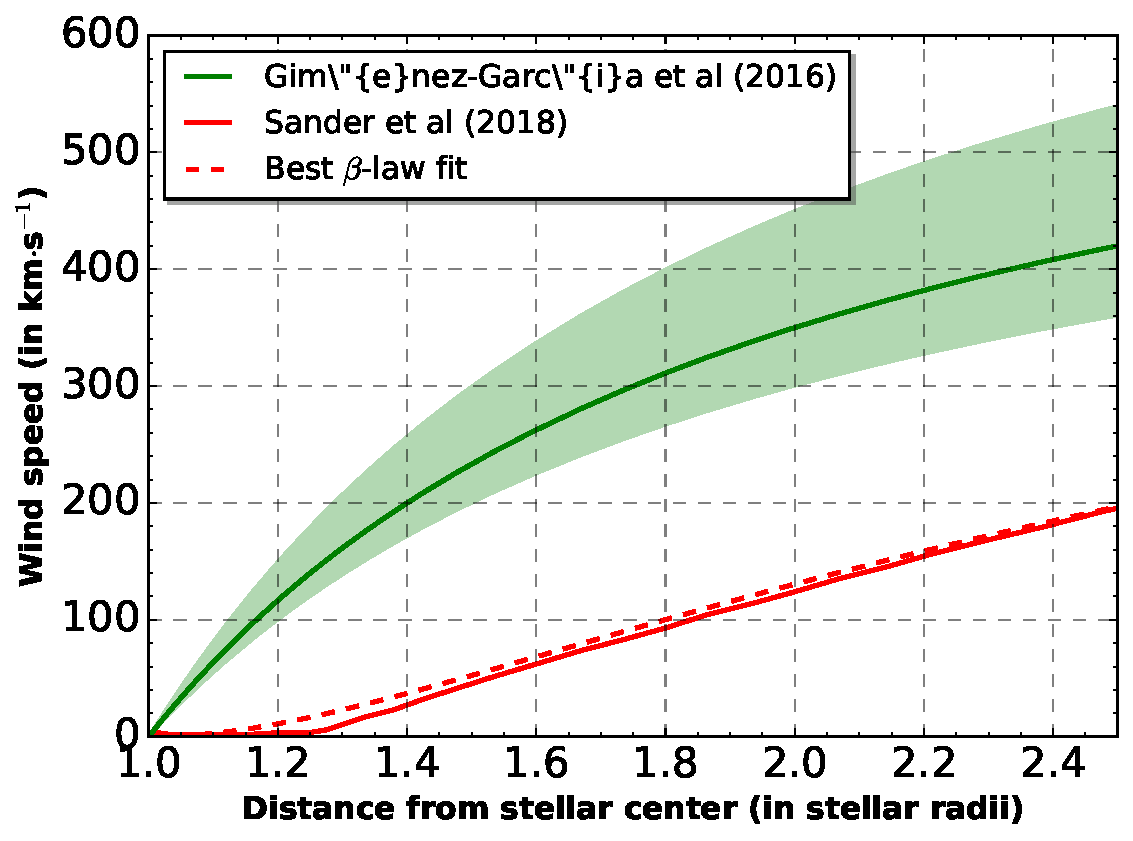
\includegraphics[width=0.99\columnwidth]{Pictures/vel_prof.pdf}
  \label{fig:vel_prof}
\end{subfigure}
\phantom{p}\\
\begin{subfigure}{.5\textwidth}
\centering
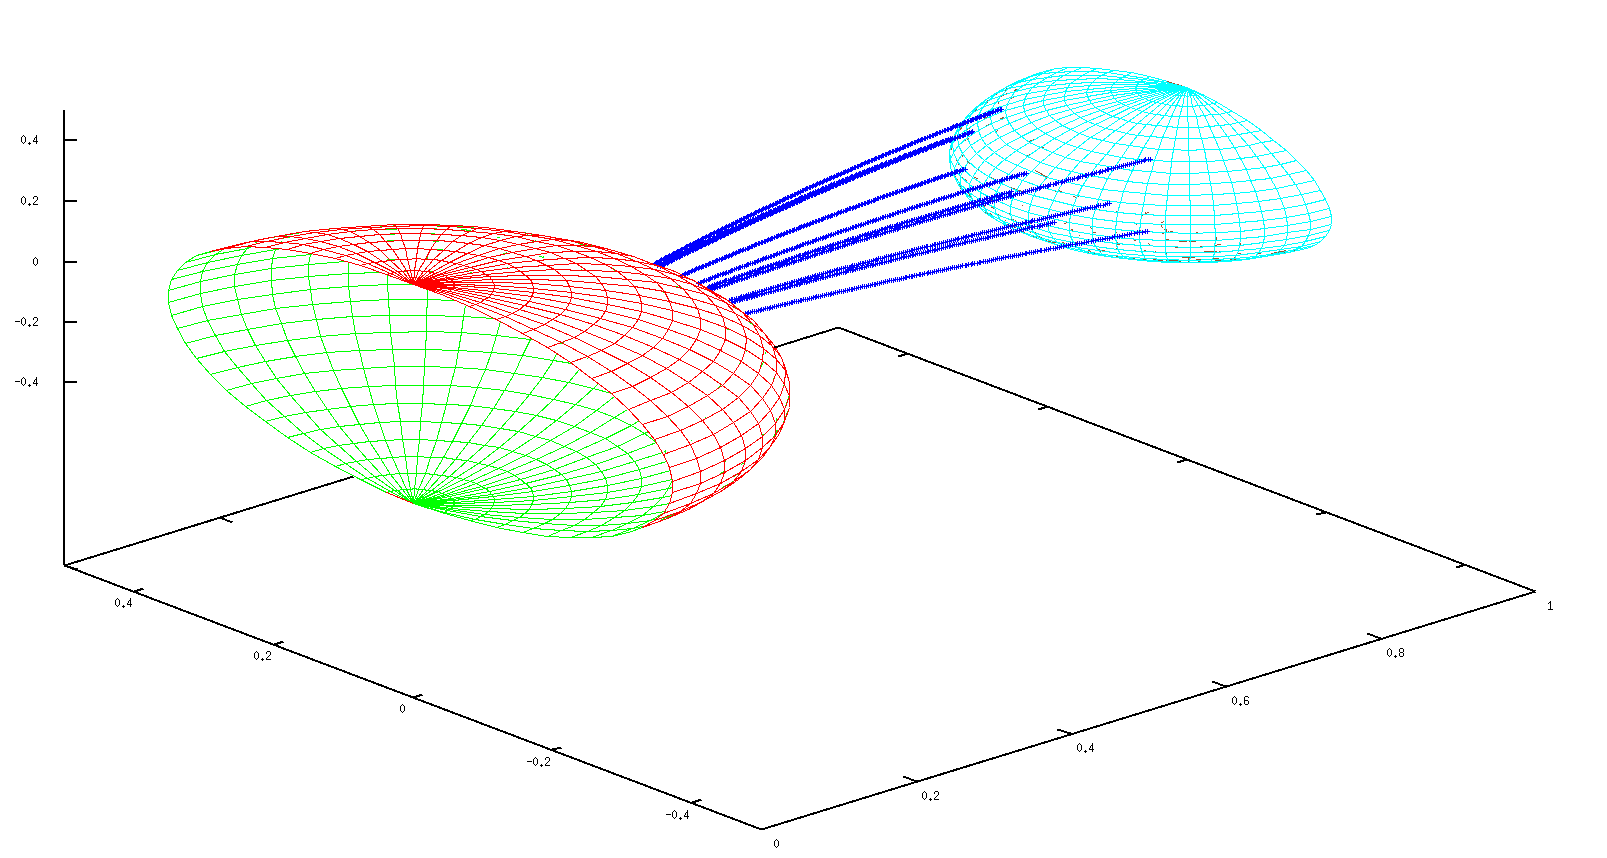
\includegraphics[width=0.99\columnwidth]{Pictures/3D.png}
  \label{fig:3D}
\end{subfigure}
\caption{(upper panel) Wind velocity profiles of a representative B0.5 Ib supergiant star, HD 77581 \citep[the donor star in Vela X-1][]{Hiltner1972,Forman1973}. The green solid line is the $\beta$-velocity profile deduced by \cite{Gimenez-Garcia2016} from observations, while the green shaded region shows the uncertainties on the terminal wind speed. \cite{Sander2017} computed the hydrodynamic atmosphere solution for the wind stratification (red solid line), here fitted by a $\beta$-velocity profile (dashed red line). (lower panel) Illustration of the integration of the streamlines (orange) from the stellar surface (blue) to the Roche lobe of the accretor (transparent green).}
\label{fig:setup}
\end{figure} 

% - - - - - - - - - - - - - - - - - - - - - - - - 
\subsection{Empirical proxy to deduce acceleration from beta-laws}
\label{sec:}
% - - - - - - - - - - - - - - - - - - - - - - - - 

% - - - - - - - - - - - - - - - - - - - - - - - - 
\subsection{The equation of motion}
\label{sec:}
% - - - - - - - - - - - - - - - - - - - - - - - - 

% ------------------------------------------------
\section{Mass transferred via wind-RLOF}
\label{sec:}
% ------------------------------------------------

We differentiate 3 mass rates : $\dot{M}$, \mdotstar and \mdotacc

in the sense of “entering the effective region of accretion" (either Roche lobe of the accretor or set by the accretion radius). Upper limit. For fast wind, effective cross-section set by accretion radius which decreases quickly and much below the radius of the Roche lobe of the accretor when the speed of the wind entering the Roche lobe gets larger than the orbital speed.

% - - - - - - - - - - - - - - - - - - - - - - - - 
\subsection{Fraction of stellar wind available for accretion}
\label{sec:}
% - - - - - - - - - - - - - - - - - - - - - - - - 

\begin{figure*}[!b]
\centering
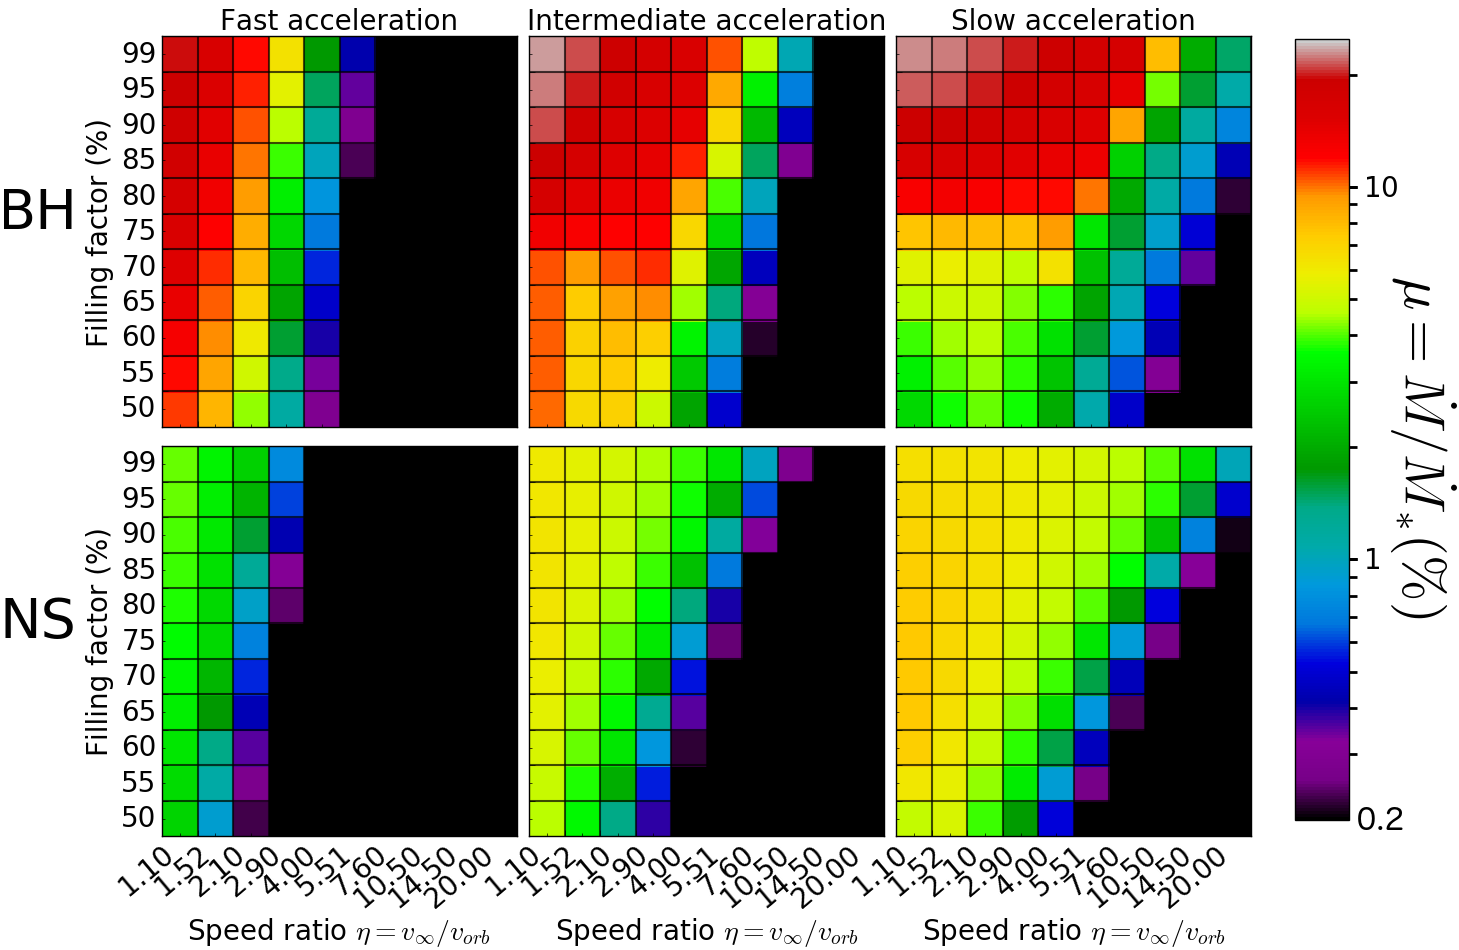
\includegraphics[width=2\columnwidth]{Pictures/mdot_grid.png}
\caption{Logarithmic color maps of the fraction of stellar wind captured by the accretor as a function of the stellar filling factor and of the ratio of the terminal wind speed by the orbital speed. From left to right, the $\beta$ exponent is 1, 2 and 3, which means a more progressive acceleration up to the terminal speed. The first (resp. second) row stands for a mass ratio of 2 (resp. 15) which means, for a fixed 20 solar-masses supergiant donor, an accreting 10 solar-masses \bh (resp. a 1.3 solar-masses \ns).}
\label{fig:mdot}
\end{figure*} 

Mapping of the stellar surface feeding the accretor Roche lobe : contribution of the high latitudes (Fig.2 : the Mollweide projection)

\% of stellar mass loss rate entering the accretor Roche lobe (Fig.3)
1st row is M101? Or Cyg X-1?
2nd row is P13?

A comparison to BHL formula (Fig.4)

% - - - - - - - - - - - - - - - - - - - - - - - - 
\subsection{Accretion luminosity}
\label{sec:}
% - - - - - - - - - - - - - - - - - - - - - - - - 

\begin{center}
\begin{table}[!h]
\caption{Scaled X-ray luminosity of a classic \sgx (Vela X-1) and of a \ulx (P13) assuming a similar fraction of the wind captured of $\sim$ 5\% obtained with $q=15$, $f=95\%$, $\beta=2$ and $\eta=2$.}
\label{tab:params}
\centering
\begin{tabularx}{0.83\columnwidth}{c|c|c}
   & Vela X-1 & P13 \\
  \hline
  $\dot{M}/\dot{M}_{\text{\mystar}}$ & \multicolumn{2}{c}{$\sim$ 5\%} \\
  \hline
  $\dot{M}_{acc}/\dot{M}$ & 4\%  & 40\% \\
  $\zeta=L_X/\dot{M}_{acc}c^2$ & 10\% & 10\% \\
  \mdotstar & 5$\cdot$10$^{-7}$M$_{\odot}\cdot$yr$^{-1}$ & 10$^{-4}$M$_{\odot}\cdot$yr$^{-1}$ \\
  $L_X$ & 5$\cdot$10$^{36}$erg$\cdot$s$^{-1}$ & 10$^{40}$erg$\cdot$s$^{-1}$ \\
\end{tabularx}
\end{table}
\end{center}

Absolute values, how realistic? Indeed, capturing a large fraction of the wind from the donor star is a necessary condition to reach significant mass transfer rates, but it is not a guarantee. For instance, Vela X-1 : ...

Mass loss rates from \cite{Vink2000,Vink2001} (Sanders, private communication).

For M101, assuming the mass of 20\msun for the Wolf-Rayet derived from the mass-luminosity relation is accurate, the total mass of the system ranges from 25\msun for an edge-on inclination to 40\msun for a 20 degrees inclination. It leads to orbital speeds approximately 3.3 to 4.2 times smaller than the terminal wind speed of 1,300km$\cdot$s$^{-1}$, their best fit to explain the Helium emission lines. They also compute a mass loss rate of 2$\cot$10$^{-5}$\msun$\cdot$yr$^{-1}$. But notice that the X-ray luminosity of a few 10$^{39}$erg$\cdot$s$^{-1}$ lies at the lower end of the ULX regime (similarly to P13, slightly brighter).

% ------------------------------------------------
\section{Discussion and conclusions}
\label{sec:}
% ------------------------------------------------

\begin{figure}
\centering
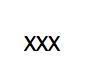
\includegraphics[width=0.99\columnwidth]{Pictures/BHL.png}
\caption{XXX}
\label{fig:BHL}
\end{figure}

In \cite{Motch2014}, it is assumed that the donor star fills its Roche lobe on the basis that the wind mass loss rate derived by \cite{Kudritzki1999} would be inferior to 10$^{-6}$erg$\cdot$s$^{-1}$. However, \cite{Kudritzki1999} did not include late type B supergiants star in their study of the wind momentum - luminosity relationship which precludes any conclusion on their mass loss rate. \cite{Vink2000} and \cite{Vink2001} provided fits for the mass loss rate and terminal speed which extend below the second bi-stability jump, for stellar effective temperatures corresponding to a B9Ia star. BUT WIND-RLOF LEADS TO SIGNIFICANT MASS TRANSFER ENHANCEMENT.

However, at these X-ray luminosities, even with an orbital period as long as in P13, we do expect a significant X-ray ionizing feedback on the wind and a serious departure from the classic wind launching mechanism \citep{Hatchett1977,Stevens1991}. \cite{Ho1987} already pinpointed that a high luminosity solution could exist when the wind was highly ionized, a result also derived by \cite{Karino2014}.

BHL

RLOF

AGB and RSG donor stars have unknown wind launching process, no report of beta-law velocity profile but low terminal speeds and large mass loss rates => could also work for them (Heida).

Suitable for Hyperluminous X-ray sources such as ESO 243-49 HLX-1, with an X-ray luminosity up to $\sim$10$^{42}$erg$\cdot$s$^{-1}$ \citep{Farrell2009,Webb2017}?

\begin{acknowledgements}
IEM is grateful to Marianne Heida, Selma De Mink and Philipp Podsiadlowski for insightful exchanges on the possible scenarios leading to ultra-luminous X-ray sources. IEM has received funding from the Research Foundation Flanders (FWO) and the European Union's Horizon 2020 research and innovation program under the Marie Sk\l odowska-Curie grant agreement No 665501. IEM and JOS thank the Instituto de F\'{i}sica de Cantabria for its hospitality and for sponsoring a meeting which brought together the massive stars and X-ray binaries communities.
% THANK REFERREE
\end{acknowledgements}

%-------------------------------------------------------------------
XXX

\bibliographystyle{aa} %agsm}
\begin{tiny}
\bibliography{/Users/Ileyk/Documents/Bibtex/article_ULX}
\end{tiny}

\end{document}